\documentclass{article}
\usepackage[letterpaper,margin=3cm]{geometry} 
\usepackage{graphicx} % Required for inserting images
\usepackage[spanish]{babel}
\usepackage[usenames]{color}
\usepackage{hyperref}
\hypersetup{colorlinks=true, linkcolor = black, citecolor= black}
\usepackage{booktabs}
\usepackage{natbib}
\usepackage{tikz}
\usepackage{float} % para usar la opción [H]
\bibliographystyle{agsm} 
\usepackage{diagbox} % Para la línea diagonal
\usepackage{listings}
\usepackage{xcolor} % Paquete para definir y usar colores
\usepackage{parskip}
\usepackage{fancyhdr}
\usepackage{amsmath}
\usepackage{titlesec}
\usepackage{lipsum}  % Solo para texto de relleno

% Configuración de fancyhdr
\pagestyle{fancy} % Usa el estilo fancyhdr
\fancyhf{} % Borra todos los encabezados y pies de página

\renewcommand{\headrulewidth}{0pt}
\renewcommand{\footrulewidth}{0pt} % Desactiva la línea horizontal predeterminada en el pie

\fancyhead[L]{\raisebox{0.20cm}{\textbf{Métodos Computacionales en Obras Civiles}}}
\fancyhead[R]{\raisebox{0.1cm}{
\includegraphics[width=0.25\linewidth]{logo principal.jpg}}}
\fancyhead[C]{\rule{\textwidth}{0.6pt}}
\fancyfoot[C]{\rule{\textwidth}{0.6pt}}
\fancyfoot[R]{\raisebox{-1.5\baselineskip}{\thepage}}

% Ajustes de geometría
% Ajustes de geometría
\geometry{
  top=3.5cm, % Aumenta el espacio en la parte superior para subir el encabezado
  bottom=2.5cm,
  headheight=2.5cm % Aumenta la altura del encabezado si es necesario
}

% Redefinir comando part
\titleclass{\part}{top} % Make part like a class
\titleformat{\part}[display]
  {\normalfont\huge\bfseries\centering}{\thepart}{20pt}{\Huge}
\titlespacing*{\part}{172.5pt}{-60pt}{10pt}
\titleformat{\part}
  {\normalfont\huge\bfseries}{}{0pt}{}

% Asegúrate de usar esto para mantener el estilo en las páginas de las partes
\titleformat{\part}[display]
  {\normalfont\huge\bfseries}{}{0pt}{}
  [\thispagestyle{fancy}] % Aplica el estilo fancy a las páginas de las partes


% Definición de colores al estilo Visual Studio Code
\definecolor{codegreen}{rgb}{0.25,0.49,0.48} % Comentarios
\definecolor{codegray}{rgb}{0.5,0.5,0.5} % Números y anotaciones
\definecolor{codepurple}{rgb}{0.58,0,0.82} % Palabras clave
\definecolor{backcolour}{rgb}{0.95,0.95,0.92} % Color de fondo

% Configuración del estilo de las celdas de código
\lstset{
    backgroundcolor=\color{backcolour},   % color de fondo; necesita que el paquete color o xcolor esté cargado
    commentstyle=\color{codegreen},       % estilo de comentarios
    keywordstyle=\color{codepurple},      % estilo de palabras clave
    numberstyle=\tiny\color{codegray},    % estilo de los números de línea
    stringstyle=\color{red},              % estilo de las cadenas de texto
    basicstyle=\ttfamily\small,           % estilo del texto básico
    breakatwhitespace=false,              % ajustes de líneas sólo en espacios en blanco
    breaklines=true,                      % ajustar las líneas si son muy largas
    captionpos=b,                         % posición de la leyenda (abajo)
    keepspaces=true,                      % preserva los espacios en el texto; útil si se usa monoespaciado
    numbers=left,                         % dónde poner los números de línea
    numbersep=5pt,                        % qué tan lejos están los números de línea del código
    showspaces=false,                     % mostrar espacios con subrayados particulares; reemplaza 'showstringspaces'
    showstringspaces=false,               % subrayar los espacios dentro de las cadenas solo
    showtabs=false,                       % mostrar tabulaciones en el código con subrayados particulares
    tabsize=2,                            % tamaños de tabulación a 2 espacios
    language=TeX,                         % lenguaje del código
    morecomment=[l]\#,                    % reconocer # como inicio de comentario en Python
    frame=single,                         % agregar un marco simple alrededor del código
    rulecolor=\color{black}               % color del marco
}



\begin{document}
%----------------------------------------------------------------------------------------
% PORTADA
%----------------------------------------------------------------------------------------
\begin{titlepage}%Inicio de la carátula, solo modificar los datos necesarios
\newcommand{\HRule}{\rule{\linewidth}{0.5mm}} 
\center 
%----------------------------------------------------------------------------------------
%	ENCABEZADO
%----------------------------------------------------------------------------------------
\includegraphics[width=10cm]{Logo principal.jpg}\\ % Si esta plantilla se copio correctamente, va a llevar la imagen del logo de la facultad.OBS: Es necesario incluir el paquete: graphicx
\vspace{3cm}
%----------------------------------------------------------------------------------------
%	SECCION DEL TITULO
%----------------------------------------------------------------------------------------
\HRule \\[0.4cm]
{ \huge \bfseries Entrega 0}\\[0.4cm] % Titulo del documento
{ \huge \bfseries Metodos Computacionales en OOCC, IOC 4201}\\[0.4cm] % Titulo del documento
\HRule \\[1.5cm]
 \vspace{5cm}
%----------------------------------------------------------------------------------------
%	SECCION DEL AUTOR
%----------------------------------------------------------------------------------------
\begin{flushright}
    { \textbf{Profesor:}
    Patricio Moreno\\
    \vspace{0.2cm}
    \textbf{Ayudante:}
    Maximiliano Biasi\\
    \vspace{0.2cm}
    \textbf{Alumno:}
    Bernardo Caprile Canala-Echevarría\\
}
\end{flushright}
\vspace{1cm}
%----------------------------------------------------------------------------------------
%	SECCION DE LA FECHA
%----------------------------------------------------------------------------------------
{\large \textbf{\today}}\\[2cm] % El comando \today coloca la fecha del dia, y esto se actualiza con cada compilacion, en caso de querer tener una fecha estatica, reemplazar el \today por la fecha deseada
\end{titlepage}
%----------------------------------------------------------------------------------------
%  INDICE
%----------------------------------------------------------------------------------------
\newpage
\tableofcontents
\newpage

%----------------------------------------------------------------------------------------
\part{Entrega 0}
\section{Introducción}
Para obras en las que se debe construir a nivel subacuático o con un nivel freático alto, es necesario el uso de ataguías. Estas estructuras temporales permiten construir de forma segura y eficiente en condiciones de humedad. Es importante, antes de instalar las ataguías, tener conocimiento de la profundidad a la que se van a hundir, la presión que se va a contener, tanto del agua como de otros factores, y la cantidad de agua que se va a bombear. De lo contrario, se pondría en riesgo la vida de los trabajadores y la maquinaria. \\

Por ello, en esta entrega se presentarán esquemas de redes de flujo, caudales de infiltración, presiones de poros y netas en ataguía, gradientes hidráulicos máximos, determinar si falla por licuefacción y calcular un factor de seguridad, de tres casos distintos de ataguías de tablaestaca. A continuación, se presenta una figura esquemática de la ataguía de tablaestaca que se analizará en esta entrega:

\begin{figure}[h!]
  \centering
  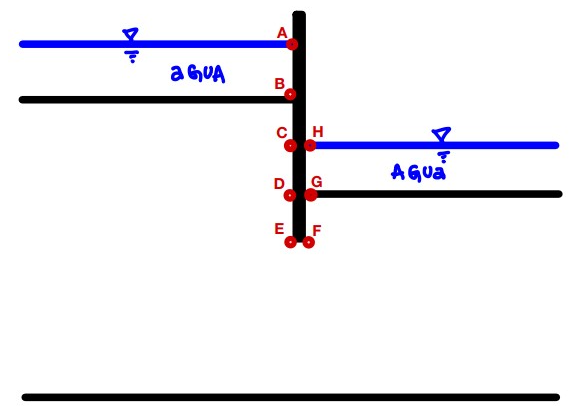
\includegraphics[width=0.8\linewidth]{graficos/puntos_interes.png}
  \caption{Esquema de la ataguía de tablaestaca}
  \label{fig:enunciado}
\end{figure}

Cabe mencionar que todos los cálculos se realizaron se encuentran en el archivo Excel del siguiente enlace: \href{https://github.com/berckanala/Proyecto-1-MCOC/tree/main/Codigos_calculos}{Cálculos}


\newpage

\section{Resultados}
\subsection{Redes de flujo}
A continuación, se muestran los esquemas de las redes de flujo de las 3 ataguías. Los esquemas a escala se pueden encontrar en el siguiente link: \href{https://github.com/berckanala/Proyecto-1-MCOC/tree/main/redes_flujo}{Esquemas ataguías}.

\begin{figure}[h]
    \centering
    \begin{minipage}{0.32\textwidth}
        \centering
        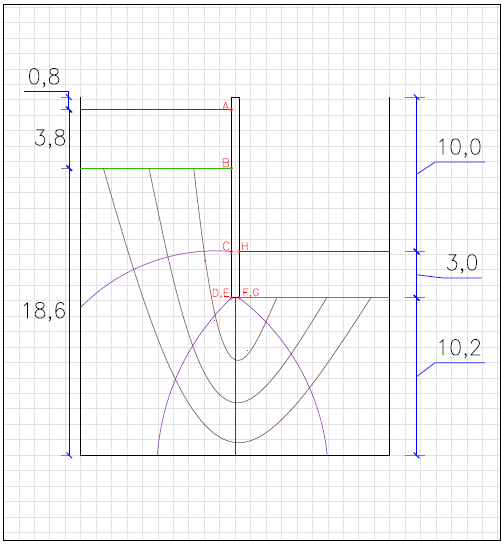
\includegraphics[width=\textwidth]{graficos/At_caso1.png}
        \caption{Ataguía con el caso 1}
        \label{fig:At_caso1}
    \end{minipage}
    \hfill
    \begin{minipage}{0.32\textwidth}
        \centering
        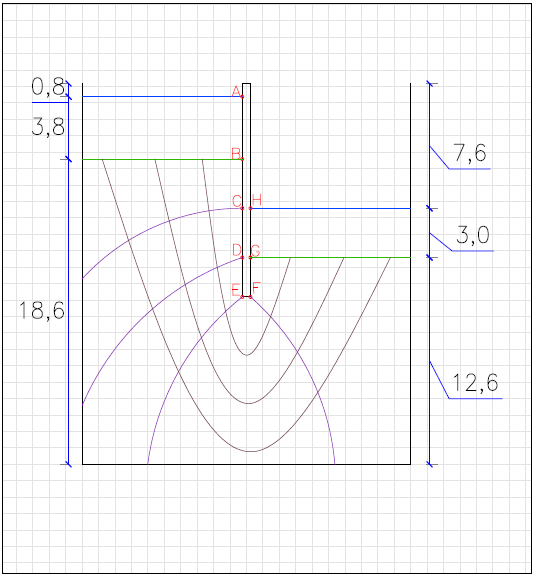
\includegraphics[width=\textwidth]{graficos/At_caso2.png}
        \caption{Ataguía con el caso 2}
        \label{fig:At_caso2}
    \end{minipage}
    \hfill
    \begin{minipage}{0.32\textwidth}
        \centering
        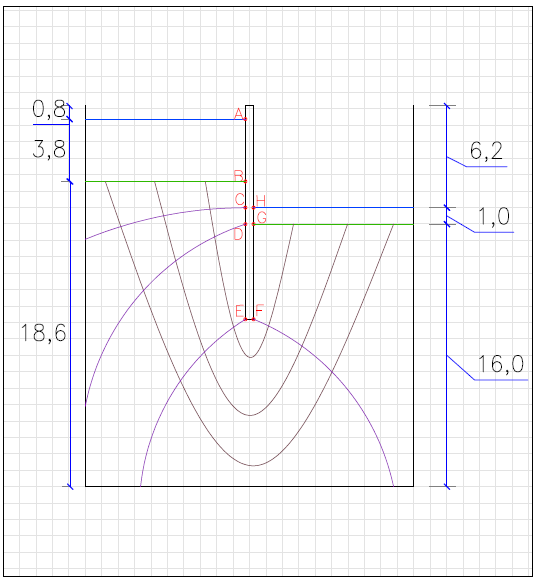
\includegraphics[width=\textwidth]{graficos/At_caso3.png}
        \caption{Ataguía con el caso 3}
        \label{fig:At_caso3}
    \end{minipage}
\end{figure}

Como se puede apreciar en la figura \ref{fig:At_caso1}, la tablaestaca no está enterrada, mientras que en la figura \ref{fig:At_caso2} la tablaestaca está enterrada a una profundidad de 2.4 metros. Por último, en la figura \ref{fig:At_caso3}, la tablaestaca está enterrada a una profundidad de 5.8 metros.

En cada esquema se utilizaron 3 líneas de flujo y 6 líneas equipotenciales. Esto corresponde a lo siguiente:

\begin{table}[h!]
  \centering
  \begin{tabular}{|c|c|}
    \hline
    Número de canales de flujo ($N_f$)& 4 \\ \hline
    Número de canales equipotenciales ($N_d$) & 5 \\ \hline
  \end{tabular}
  \caption{Número de canales de flujo y equipotenciales}
\end{table}

\subsection{Caudales de infiltración}
Para poder calcular los caudales de infiltración, se ocupó la ley de Darcy, la cual se expresa de la siguiente forma:

\begin{equation}
    q = k \cdot \Delta H \cdot \frac{N_f}{N_d} \cdot 86400
\end{equation}

Donde:
\begin{itemize}
    \item $q$: Caudal de infiltración (m/s)
    \item $k$: Coeficiente de permeabilidad
    \item $\Delta H$: Diferencia de altura entre dos líneas equipotenciales (m)
\end{itemize}

\newpage

Los caudales de infiltración para cada caso se presentan en la siguiente tabla:

\begin{table}[h!]
  \centering
  \begin{tabular}{ccc}
    \hline
    \textbf{Caso} &\textbf{$\Delta H$ (m)}  &\textbf{Caudal de infiltración ($m^3/dia$)} \\
    \hline
    1 &9.2 &43.87 \\
    2 & 6.8&32.43\\
    3 &5.4 &25.75\\
    \hline
  \end{tabular}
  \caption{Caudales de infiltración}
  \label{tab:caudales}
\end{table}

Como se puede apreciar en la tabla \ref{tab:caudales}, el caudal de infiltración disminuye a medida que la tablaestaca se entierra más y la diferencia de altura va disminyendo. Sin embrago, estos valores dan cuenta de la importancia de calcular el caudal de infiltración para la correcta utilización de bombas. Ya que, si no se calcula correctamente, se podría inundar la obra con la maquinaria y trabajadores dentro.

\subsection{Presión de poros}
Para calcular la presión de poros, se utilizó el siguiente procedimiento:

Lo primero es fijar una una cota de referencia, esta se puso en la base inferior del esquema, para poder tener la energía geodésica de cada punto, a este valor lo denominaremos ($z_g$). Luego, a cada punto se le asigna un ($n_i$) este valor representa en que línea equipontecial se encuentra el punto. Cabe mencionar que el punto A y H no cuentan con una línea equipontencial. Posteriormente, se calcula la energía total en cada punto con la siguiente fórmula:

\begin{equation}
  H_i = H_0 - \frac{\Delta H}{n_p} \cdot n_i
\end{equation}

Donde:
\begin{itemize}
    \item $H_i$: Energía total en el punto i (m)
    \item $H_0$: Energía total en la cota de referencia (m)
    \item $\Delta H$: Diferencia de altura entre dos líneas equipotenciales (m)
    \item $n_p$: Número de canales equipotenciales
    \item $n_i$: Número de la línea equipotencial en la que se encuentra el punto i
\end{itemize}

Finalmente, se calcula la presión de poros con la siguiente fórmula:

\begin{equation}
  u_i =  (H_i - z_g)\cdot \frac{\gamma_w}{1000}
\end{equation}

Donde:
\begin{itemize}
    \item $u_i$: Presión de poros en el punto i (kPa)
    \item $\gamma_w$: Peso específico del agua (N/m$^3$)
\end{itemize}

\newpage

A continuación, se presentan las presiones de poros para cada caso:

\begin{table}[h!]
  \centering
  \begin{tabular}{ccccc}
    \hline
    \textbf{Punto} & \textbf{Altura geodésica (m)} & \textbf{$n_i$} & \textbf{$H_i$} & \textbf{Presión de poros (kPa)} \\
    \hline
    A & 22.4 & - & - &0 \\
    B & 18.6 &  0 & 22.4 &37.278 \\
    C & 13.2 & 1  & 10.56 &72.20 \\
    D & 10.2&  2 & 18.72 &83.58 \\
    E & 10.2 & 3  & 16.88 &65.53 \\
    F & 10.2 & 4  & 15.04 & 47.48\\
    G & 10.2 & 5  & 13.02 &29.43 \\
    H & 13.2 & - & - &0 \\
    \hline
  \end{tabular}
  \caption{Presiones de poros en el caso 1}
  \label{tab:presion1}
\end{table}


\begin{table}[h!]
  \centering
    \begin{tabular}{cccccc}
    \hline
    \textbf{Punto} & \textbf{Altura geodésica (m)} & \textbf{$n_i$} & \textbf{$H_i$} & \textbf{Presión de poros (kPa)} \\
    \hline
    A &  22,4 & - & - & 0  \\ 
    B &  18,6 & 0 & 22,4 & 37,278  \\ 
    C &  15,6 & 1 & 21,04 & 53,3664  \\ 
    D &  12,6 & 2 & 19,68 & 69,4548  \\ 
    E &  10,2 & 3 & 18,32 & 79,6572  \\ 
    F &  10,2 & 4 & 16,96 & 66,3156  \\ 
    G &  12,6 & 5 & 15,6 & 29,43  \\ 
    H &  15,6 & - & - & 0  \\ \hline
    \end{tabular}
  \caption{Presiones de poros en el caso 2}
  \label{tab:presion2}
\end{table}
  
\begin{table}[h!]
    \centering
      \begin{tabular}{cccccc}
      \hline
      \textbf{Punto} & \textbf{Altura geodésica (m)} & \textbf{$n_i$} & \textbf{$H_i$} & \textbf{Presión de poros (kPa)} \\ \hline
      A &  22,4 & - & - & 0 \\ 
      B &  18,6 & 0 & 22,4 & 37,278 \\ 
      C & 17 & 1 & 21,32 & 42,3792 \\ 
      D & 16 & 2 & 20,24 & 41,5944 \\ 
      E &  10,2 & 3 & 19,16 & 87,8976 \\ 
      F &  10,2 & 4 & 18,08 & 77,3028 \\ 
      G & 16 & 5 & 17 & 9,81 \\ 
      H & 17 & - & - & 0 \\ \hline
      \end{tabular}
    \caption{Presiones de poros en el caso 3}
    \label{tab:presion3}
\end{table}
    
Lo que es importante ver es la diferencia de presion de poros entre los puntos A y G, ya que, dependiendo esta diferencia la inflitración influye en el caudal de inflitración. Como se puede observar, el la tabla \ref{tab:presion1} la presión en G es de 29.43 kPa, mientras que en la tabla \ref{tab:presion2} es de 29.43 kPa y en la tabla \ref{tab:presion3} es de 9.81 kPa. Esto se debe a que en el caso 1 y 2 la altura del agua es la misma y en el caso 3 la tablaestaca está más enterrada, lo que disminuye la presión de poros en el punto G.

\newpage

\subsection{Presiones netas en la ataguía}
Para calcular las presiones netas en la ataguía, se restan las presiones que están en la misma altura, quedando la siguiente tabla:

\begin{table}[h!]
  \centering
  \begin{tabular}{cc}
    \hline
    \textbf{Caso} & \textbf{Presión neta en la ataguía (kPa)} \\
    \hline
    A & 0 \\
    B & 37.278 \\
    C & 72.2 \\
    D-E & 54.15\\
    F-G & 18.05 \\
    \hline  
  \end{tabular}
  \caption{Presiones netas en la ataguía caso 1}
  \label{tab:presion_neta1}
\end{table}

\begin{table}[h!]
  \centering
  \begin{tabular}{cc}
    \hline
    \textbf{Caso} & \textbf{Presión neta en la ataguía (kPa)} \\
    \hline
    A & 0 \\
    B & 37.278 \\
    C & 53.36 \\
    D-E & 40.02\\
    F-G & 13.34 \\
    \hline  
  \end{tabular}
  \caption{Presiones netas en la ataguía caso 2}
  \label{tab:presion_neta2}
\end{table}

\begin{table}[h!]
  \centering
  \begin{tabular}{cc}
    \hline
    \textbf{Caso} & \textbf{Presión neta en la ataguía (kPa)} \\
    \hline
    A & 0 \\
    B & 37.278 \\
    C & 42.38 \\
    D-E & 31.78\\
    F-G & 10.59 \\
    \hline  
  \end{tabular}
  \caption{Presiones netas en la ataguía caso 3}
  \label{tab:presion_neta3}
\end{table}

Con las presiones netas se puede ver como la presión neta disminuye de forma significativa a medida que la tablaestaca se entierra más. Esto hace que la tablaestaca sea más estable y no se desplace por la presión del agua. Además, se puede observar que el punto crítico en términos de presión es el punto C es el más crítico, ya que ahí es donde empieza el agua a ejercer presión por dentro en la tablaestaca.


\subsection{Máximo gradiente hidráulico}

Para calcular el máximo gradiente hidráulico, se utilizó la siguiente fórmula:

\begin{equation}
  i_{max} = \frac{\Delta H}{L_{min}}
\end{equation}

Donde:
\begin{itemize}
    \item $i_{max}$: Máximo gradiente hidráulico 
    \item $\Delta H$: Diferencia de altura entre dos líneas equipotenciales (m)
    \item $L_{min}$: Distancia mínima entre dos líneas de flujo (m)
\end{itemize}


\begin{table}[h!]
  \centering
  \begin{tabular}{cc}
    \hline
    \textbf{Caso} & \textbf{Máximo gradiente hidráulico} \\
    \hline
    1 & 1.095 \\
    2 & 0.63 \\
    3 & 0.38 \\
    \hline
  \end{tabular}
  \caption{Máximo gradiente hidráulico}
  \label{tab:gradiente}
\end{table}

Como se puede observar en la tabla \ref{tab:gradiente}, el máximo gradiente hidráulico disminuye a medida que la tablaestaca se entierra más. Esto se debe a que la distancia entre las líneas de flujo aumenta junto con que la diferencia de altura del agua va disminuyendo, lo que hace que el gradiente hidráulico sea menor. 

\subsection{Falla por licuefacción}

Para determinar si la tablaestaca falla por licuefacción, se calculó el gradiente hidráulico crítico con la siguiente fórmula:

\begin{equation}
  i_{crit} = \frac{\gamma_{sat}-\gamma_w}{\gamma_w} 
\end{equation}

Donde:
\begin{itemize}
    \item $i_{crit}$: Gradiente hidráulico crítico
    \item $\gamma_{sat}$: Peso específico saturado del suelo (N/m$^3$)
    \item $\gamma_w$: Peso específico del agua (N/m$^3$)  
\end{itemize}
Luego, si este valor, que es constante para todos los casos, es menor al gradiente hidráulico máximo de cada caso se puede afirmar que la tablaestaca falla por licuefacción. A continuación, se presenta una tabla con los resultados:

\begin{table}[h!]
  \centering
  \begin{tabular}{cccc}
    \hline
    \textbf{Caso} & \textbf{Máximo gradiente hidráulico}& \textbf{Gradiente hidráulico crítico} &\textbf{Falla por licuefacción} \\
    \hline
    1 &1.095 & 1.14 &No \\
    2 &0.63  & 1.14 &No \\
    3 &0.38  & 1.14 &No \\
    \hline
  \end{tabular}
  \caption{Falla por licuefacción}
  \label{tab:licuefaccion}
\end{table}

Como se puede apreciar, el caso más cercano a la falla es el caso 1, esto es debido a que la tablaestaca no está enterrada, lo que hace que el gradiente hidráulico sea mayor. Sin embargo, en todos los casos el gradiente hidráulico crítico es mayor al máximo, por lo que no hay falla por licuefacción. Estos resultados demuestran que a mayor profundidad de la tablaestaca, menor es el riesgo de falla por licuefacción.

\newpage
\subsection{Factor de seguridad}
Para poder calcular el factor de seguridad, se utilizó la siguiente fórmula:

\begin{equation}
  FS = \frac{i_{crit}}{i_{max}}
\end{equation}

Donde:
\begin{itemize}
    \item $FS$: Factor de seguridad
\end{itemize}

A continuación, se presenta una tabla con los resultados:

\begin{table}[h!]
  \centering
  \begin{tabular}{cc}
    \hline
    \textbf{Caso} & \textbf{Factor de seguridad} \\
    \hline
    1 &1.04 \\
    2 &1.81 \\
    3 &3.00 \\
    \hline
  \end{tabular}
  \caption{Factor de seguridad}
  \label{tab:seguridad}
\end{table}

Tal como se dijo anteriormente, a medida que la tablaestaca esta más enterrada la ataguía es más segura. Ocupando las cotas que se pueden apreciar en las figuras (\ref{fig:At_caso1}, \ref{fig:At_caso2} y \ref{fig:At_caso3}) el pasar de 0 metros de profundidad a 5.8 metros de profundidad, el factor de seguridad aumenta de 1.04 a 3.00. Esto demuestra la importancia de enterrar la tablaestaca a una profundidad adecuada para evitar fallas en la ataguía. 

\newpage

\section{Conclusiones}

En conclusión, se puede decir que la ataguía de tablaestaca es una estructura que permite construir de forma segura y eficiente en condiciones de humedad. Sin embargo, es necesario prestar atención a la profundidad a la que esta se va a enterrar, ya que esto influye en la presión de poros, el gradiente hidráulico y el factor de seguridad. En este sentido, se puede concluir que a mayor profundidad de la tablaestaca, menor es el riesgo de falla por licuefacción y mayor es el factor de seguridad. Por lo tanto, es importante realizar los cálculos necesarios para determinar la profundidad adecuada de la tablaestaca y así evitar posibles accidentes en la obra.\\

Finalmente, se concluye que el caso 1 es el más inestable de los tres, ya que la tablaestaca no está enterrada, mientras el caso 3 es el más estable, ya que la tablaestaca está enterrada a una profundidad de 5.8 metros. La diferencia entre estos dos casos se pudo notar en todos los cálculos realizados, por ejemplo, en el caso 1 tiene mayor caudal de infiltración, mayor presión neta en la tablaestaca, mayor gradiente hidráulico máximo y un tercio del factor de seguridad del caso 3.

\end{document}